\documentclass[a4paper,11pt,fleqn]{article}\usepackage[]{graphicx}\usepackage[]{color}
%% maxwidth is the original width if it is less than linewidth
%% otherwise use linewidth (to make sure the graphics do not exceed the margin)
\makeatletter
\def\maxwidth{ %
  \ifdim\Gin@nat@width>\linewidth
    \linewidth
  \else
    \Gin@nat@width
  \fi
}
\makeatother

\definecolor{fgcolor}{rgb}{0, 0, 0}
\newcommand{\hlnum}[1]{\textcolor[rgb]{0,0,0}{#1}}%
\newcommand{\hlstr}[1]{\textcolor[rgb]{0,0,0}{#1}}%
\newcommand{\hlcom}[1]{\textcolor[rgb]{0.4,0.4,0.4}{\textit{#1}}}%
\newcommand{\hlopt}[1]{\textcolor[rgb]{0,0,0}{\textbf{#1}}}%
\newcommand{\hlstd}[1]{\textcolor[rgb]{0,0,0}{#1}}%
\newcommand{\hlkwa}[1]{\textcolor[rgb]{0,0,0}{\textbf{#1}}}%
\newcommand{\hlkwb}[1]{\textcolor[rgb]{0,0,0}{\textbf{#1}}}%
\newcommand{\hlkwc}[1]{\textcolor[rgb]{0,0,0}{\textbf{#1}}}%
\newcommand{\hlkwd}[1]{\textcolor[rgb]{0,0,0}{\textbf{#1}}}%
\let\hlipl\hlkwb

\usepackage{framed}
\makeatletter
\newenvironment{kframe}{%
 \def\at@end@of@kframe{}%
 \ifinner\ifhmode%
  \def\at@end@of@kframe{\end{minipage}}%
  \begin{minipage}{\columnwidth}%
 \fi\fi%
 \def\FrameCommand##1{\hskip\@totalleftmargin \hskip-\fboxsep
 \colorbox{shadecolor}{##1}\hskip-\fboxsep
     % There is no \\@totalrightmargin, so:
     \hskip-\linewidth \hskip-\@totalleftmargin \hskip\columnwidth}%
 \MakeFramed {\advance\hsize-\width
   \@totalleftmargin\z@ \linewidth\hsize
   \@setminipage}}%
 {\par\unskip\endMakeFramed%
 \at@end@of@kframe}
\makeatother

\definecolor{shadecolor}{rgb}{.97, .97, .97}
\definecolor{messagecolor}{rgb}{0, 0, 0}
\definecolor{warningcolor}{rgb}{1, 0, 1}
\definecolor{errorcolor}{rgb}{1, 0, 0}
\newenvironment{knitrout}{}{} % an empty environment to be redefined in TeX

\usepackage{alltt}

%%----------------------------------------------------------------------
%% opções comuns
\usepackage[brazilian]{babel}
\usepackage[utf8]{inputenc}
\usepackage[T1]{fontenc}
\usepackage{textcomp}
%\usepackage[margin=2cm]{geometry}
\usepackage{indentfirst}
\usepackage{fancybox}
%\usepackage[usenames,dvipsnames]{color}
\usepackage{amsmath,amsfonts,amssymb,amsthm}
\usepackage{lscape}
\usepackage{natbib}
\setlength{\bibsep}{0.0pt}
\usepackage{url}
\usepackage{multicol}
\usepackage{multirow}
\usepackage[final]{pdfpages}
\usepackage{setspace}
\usepackage{paralist} % enumitem, compactitem
%%----------------------------------------------------------------------

%%----------------------------------------------------------------------
%% FLOATS: graficos e tabelas
\usepackage{graphicx}
\usepackage{float} % fornece a opção [H] para floats
\usepackage{longtable}
\usepackage{supertabular}
%% captions e headings em sans-serif
\usepackage[font={sf},labelfont={sf,bf}]{caption}
\usepackage{subcaption}
\renewcommand{\thesubfigure}{\Alph{subfigure}}
\usepackage{titlesec}
\titleformat*{\section}{\normalsize\bfseries\sffamily}
\titleformat*{\subsection}{\normalsize\bfseries\sffamily}
\titleformat*{\subsubsection}{\normalsize\bfseries\sffamily}
\titleformat*{\paragraph}{\normalsize\bfseries\sffamily}
\titleformat*{\subparagraph}{\normalsize\bfseries\sffamily}
\theoremstyle{definition}
\newtheorem*{mydef}{Definição}
%%----------------------------------------------------------------------

%%----------------------------------------------------------------------
%% definiçoes de hyperref e xcolor
\usepackage{hyperref}
\usepackage{xcolor}
%%----------------------------------------------------------------------

%%----------------------------------------------------------------------
%% FONTES

%% micro-tipografia
\usepackage[protrusion=true,expansion=true]{microtype}
%% Bitstream Charter with mathdesign
\usepackage{lmodern} % sans-serif: Latin Modern
\usepackage[charter]{mathdesign} % serif: Bitstream Charter
\usepackage[scaled]{beramono} % truetype: Bistream Vera Sans Mono
\usepackage[scaled]{helvet}
%\usepackage{inconsolata}


%\usepackage[sf]{titlesec}
%%----------------------------------------------------------------------

%%----------------------------------------------------------------------
%% hifenização
\usepackage[htt]{hyphenat} % permite hifenizar texttt. Ao inves disso
% pode usar \allowbreak no ponto qu quiser quebrar dentro do texttt
\hyphenation{con-si-de-ra-ção pes-que-i-ros pes-que-i-ra se-gui-do-ras
  di-fe-ren-tes pla-ni-lha pla-ni-lhão re-fe-ren-te con-ta-gem
  em-bar-ques qua-li-da-de a-le-a-to-ri-za-dos}
%%----------------------------------------------------------------------

%%----------------------------------------------------------------------
%% comandos customizados
\usepackage{xspace} % lida com os espaços depois dos comandos
\providecommand{\eg}{\textit{e.g.}\xspace}
\providecommand{\ie}{\textit{i.e.}\xspace}
\providecommand{\R}{\textsf{R}\xspace}
\newcommand{\mb}[1]{\mathbf{#1}}
\newcommand{\bs}[1]{\boldsymbol{#1}}
\providecommand{\E}{\text{E}}
\providecommand{\Var}{\text{Var}}
\providecommand{\logit}{\text{logit}}
%% Para alterar o titulo do thebibliography
\addto\captionsbrazilian{%
  \renewcommand{\refname}{Bibliografia}
}
%%----------------------------------------------------------------------

%%----------------------------------------------------------------------
%% Comandos para deixar o texto mais compacto
\usepackage{marginnote}
\usepackage[top=1cm, bottom=1cm, inner=1cm, outer=1cm,nohead, nofoot, heightrounded, marginparsep=.05cm]{geometry}
\setlength{\parindent}{0pt}
%%----------------------------------------------------------------------
\IfFileExists{upquote.sty}{\usepackage{upquote}}{}
\begin{document}

\reversemarginpar % para colocar a marginnote a esquerda





\hrule
\vspace{0.3cm}

\begin{minipage}[c]{.85\textwidth}
  Bioestatística --- CE001 \\
  Prof. Fernando de Pol Mayer --- Departamento de Estatística - DEST \\
  Exercícios: amostragem e análise exploratória de dados \\
  Nome: GABARITO  \hfill GRR: \hspace{2cm}
\end{minipage}\hfill
\begin{minipage}[c]{.15\textwidth}
\flushright

\includegraphics[width=2.2cm]{../img/ufpr-logo.png}
\end{minipage}

\vspace{0.3cm}
\hrule
\vspace{0.3cm}
%%----------------------------------------------------------------------

\begin{compactenum}[1.]
\item (\textit{Exemplo de resposta}) Do ponto de vista estatístico, uma
  população é um conjunto de indivíduos, objetos ou produtos que contém,
  em comum, a característica que temos interesse. Uma amostra é um
  subconjunto desta população, em geral com dimensões bem menores, mas
  que possui a mesma característica que temos interesse.

  Um parâmetro é alguma medida numérica que descreve alguma
  característica da população, enquanto que uma estatística é uma medida
  obtida a partir de uma amostra.

  Uma amostra representativa da população é obtida garantindo-se que o
  processo de amostragem foi realizado através de algum meio aleatório,
  garantindo com que todos os elementos da população tenham a mesma
  probabilidade de serem amostrados.
\end{compactenum}

\vspace{0.3cm}
\hrule
\vspace{0.3cm}

\begin{compactenum}[2.]
\item (a) E \quad (b) E \quad (c) P \quad (d) E \quad (e) P \quad (f)
  E \quad (g) P
\end{compactenum}

\vspace{0.3cm}
\hrule
\vspace{0.3cm}

\begin{compactenum}[3.]
\item Aleatória Simples (A), Sistemática (S), Estratificada (E) ou
  Conglomerado (C)
  \begin{compactenum}
  \item[] (a) C \quad (b) A \quad (c) S \quad (d) E \quad (e) C \quad
    (f) E
  \end{compactenum}
\end{compactenum}

\vspace{0.3cm}
\hrule
\vspace{0.3cm}

\begin{compactenum}[4.]
\item (a) C \quad (b) D \quad (c) N \quad (d) D \quad (e) C \quad (f) C
  \quad (g) O \quad (h) C \quad
\end{compactenum}

\vspace{0.3cm}
\hrule
\vspace{0.3cm}

\begin{compactenum}[5.]
\item Tabela e gráfico (em ordem alfabética)

\begin{multicols}{2}

  \begin{tabular}{cc}
    \hline
    \textbf{Área do conhecimento} & \textbf{Frequência} \\
    \hline
    A\&M & 5 \\
    CE & 4 \\
    F\&N & 7 \\
    L\& L & 6 \\
    \hline
  \end{tabular}

\columnbreak

\begin{knitrout}\small
\definecolor{shadecolor}{rgb}{1, 1, 1}\color{fgcolor}

{\centering 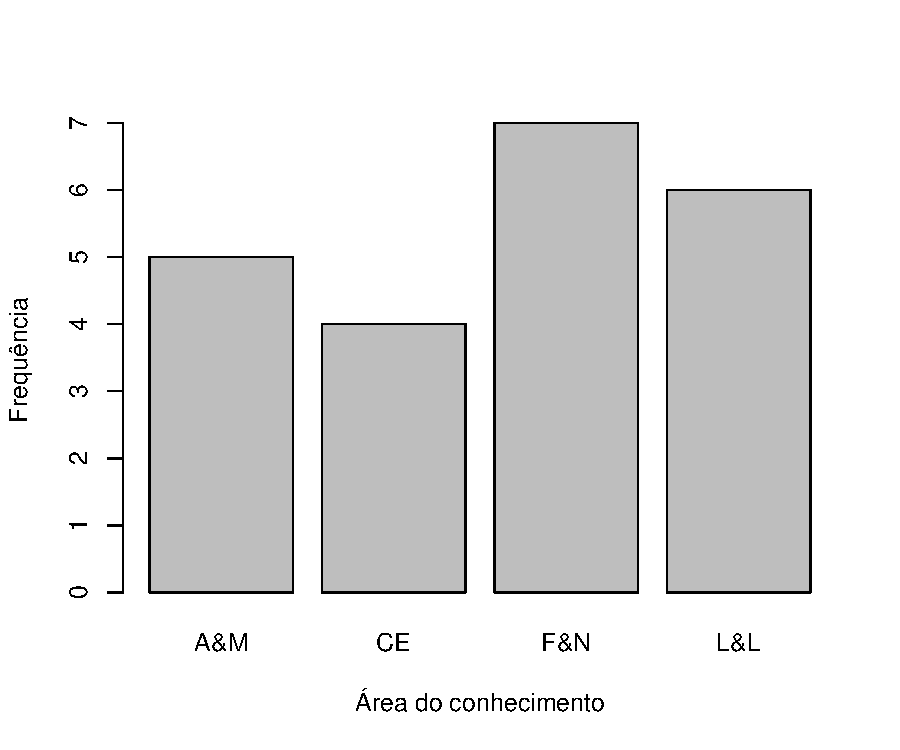
\includegraphics[width=.45\textwidth]{figure/unnamed-chunk-1-1} 

}



\end{knitrout}
\end{multicols}

\end{compactenum}

%% \vspace{0.3cm}
%% \hrule
%% \vspace{0.3cm}

\vspace{0.3cm}
\hrule
\vspace{0.3cm}

\begin{compactenum}[6.]
\item (a)

\begin{table}[h]
  \centering
  \begin{tabular}{ccccc}
    \hline
    \textbf{Classes} & \textbf{Frequência} & \textbf{Frequência
      relativa} & \textbf{Frequência acumulada} & \textbf{Frequência
      relativa acumulada} \\
    \hline
    $0,5 \vdash 1,0$ & 1   & 0,001 & 1   & 0,001 \\
    $1,0 \vdash 1,5$ & 3   & 0,004 & 4   & 0,005 \\
    $1,5 \vdash 2,0$ & 22  & 0,027 & 26  & 0,032 \\
    $2,0 \vdash 2,5$ & 115 & 0,140 & 141 & 0,172 \\
    $2,5 \vdash 3,0$ & 263 & 0,320 & 404 & 0,491 \\
    $3,0 \vdash 3,5$ & 287 & 0,349 & 691 & 0,841 \\
    $3,5 \vdash 4,0$ & 99  & 0,120 & 790 & 0,961 \\
    $4,0 \vdash 4,5$ & 32  & 0,039 & 822 & 1,000 \\
    \hline
    \textbf{Total} & 822 & 1 & & \\
    \hline
  \end{tabular}
\end{table}
\begin{compactenum}
  \item[] (b) Entre 3 e 3,5 minutos \quad (c) 49,1\%  \quad (d) 26  \quad
    (e) 3,9\%  \quad (f) 0,1\%
  \end{compactenum}
\end{compactenum}

\vspace{0.3cm}
\hrule
\vspace{0.3cm}

\clearpage

\vspace{0.3cm}
\hrule
\vspace{0.3cm}

\begin{compactenum}[7.]

\item $AMP = MAX - MIN = 69-29 = 40$, $k = \sqrt{n} = \sqrt{40} =
  6,325$, $h = \frac{AMP}{k} = \frac{40}{6,325} = 6,324$. Um exemplo de
  tabela com amplitude de classe igual a 6, e começando em 24:
% latex table generated in R 3.3.1 by xtable 1.8-2 package
% Wed Aug 31 16:54:55 2016
\begin{table}[ht]
\centering
\begin{tabular}{cccccc}
  \hline
 & Freq.abs & Freq.rel & Freq.acum & Freq.acum.rel & Dens. \\ 
  \hline
$[24,30)$ &    1 & 0,025 &    1 & 0,025 & 0,004 \\ 
  $[30,36)$ &    4 & 0,100 &    5 & 0,125 & 0,017 \\ 
  $[36,42)$ &    8 & 0,200 &   13 & 0,325 & 0,033 \\ 
  $[42,48)$ &    7 & 0,175 &   20 & 0,500 & 0,029 \\ 
  $[48,54)$ &    9 & 0,225 &   29 & 0,725 & 0,037 \\ 
  $[54,60)$ &    4 & 0,100 &   33 & 0,825 & 0,017 \\ 
  $[60,66)$ &    5 & 0,125 &   38 & 0,950 & 0,021 \\ 
  $[66,72)$ &    2 & 0,050 &   40 & 1,000 & 0,008 \\ 
   \hline
\end{tabular}
\end{table}

Histogramas:
\begin{knitrout}\small
\definecolor{shadecolor}{rgb}{1, 1, 1}\color{fgcolor}

{\centering 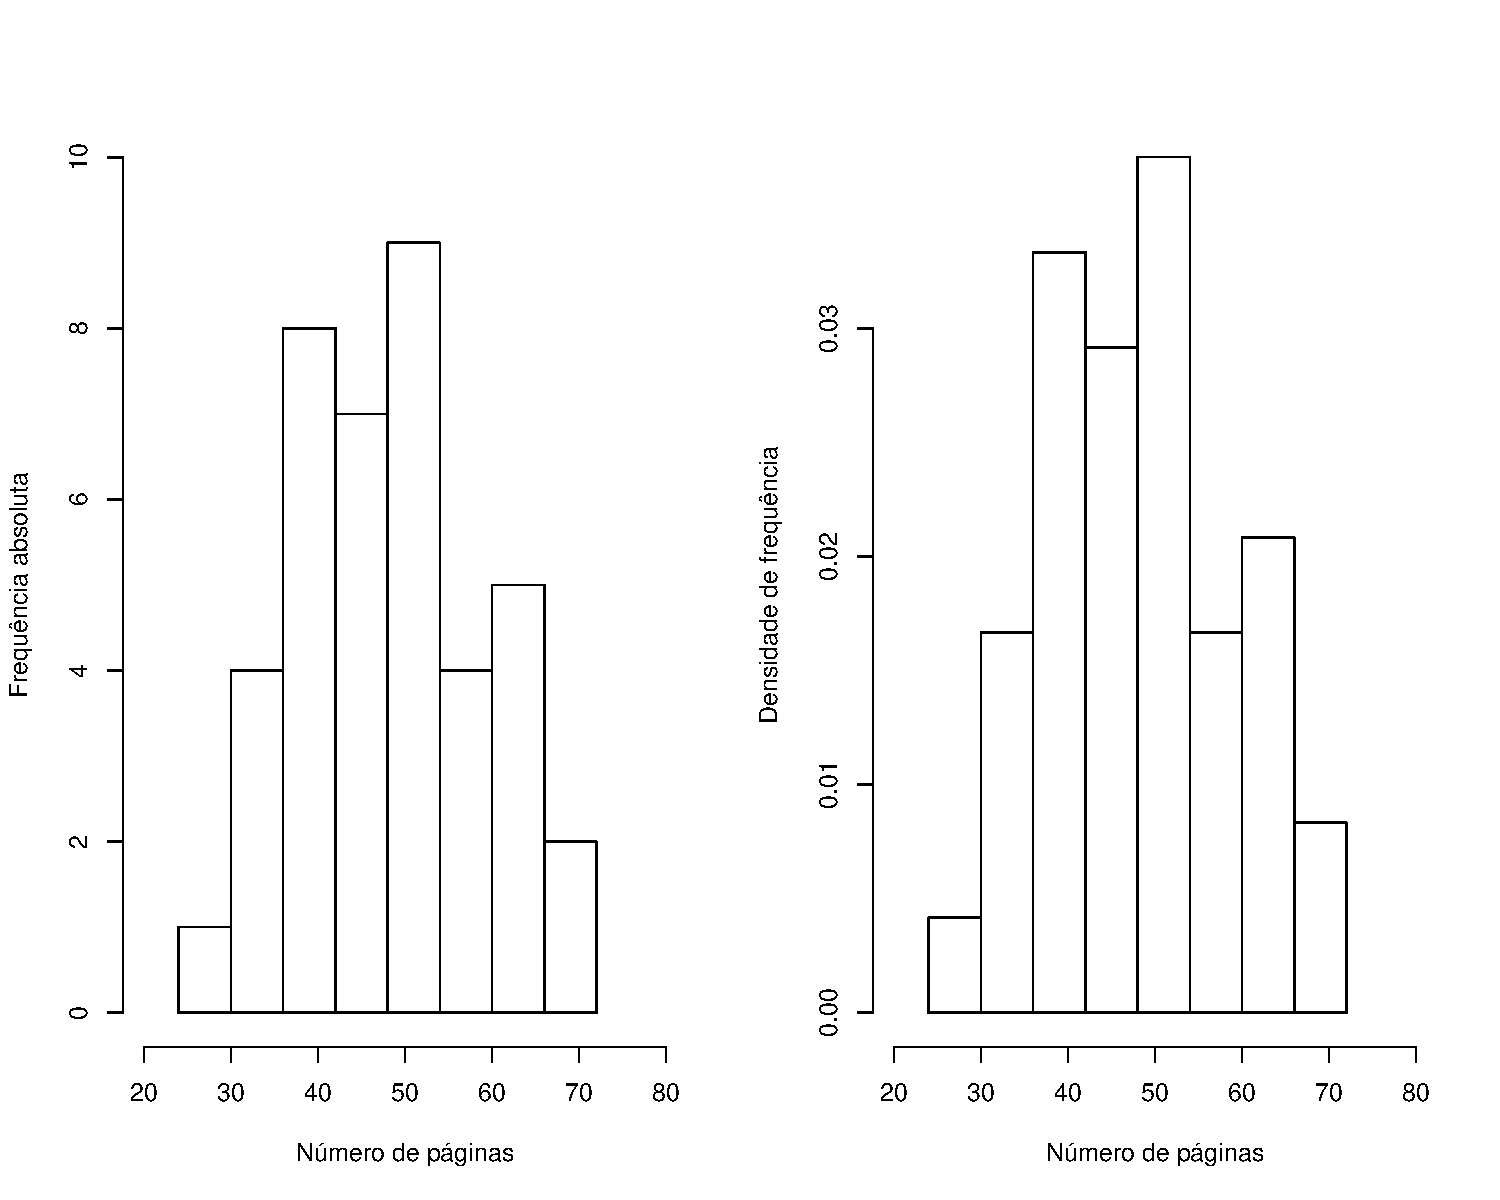
\includegraphics[width=.8\textwidth]{figure/unnamed-chunk-5-1} 

}



\end{knitrout}

Gráfico de ramo-e-folhas (uma opção):

\begin{knitrout}\small
\definecolor{shadecolor}{rgb}{1, 1, 1}\color{fgcolor}\begin{kframe}
\begin{verbatim}

  The decimal point is 1 digit(s) to the right of the |

  2 | 9
  3 | 0113
  3 | 88889
  4 | 011234
  4 | 55669
  5 | 000023334
  5 | 568
  6 | 0224
  6 | 569
\end{verbatim}
\end{kframe}
\end{knitrout}

\end{compactenum}

\vspace{0.3cm}
\hrule
\vspace{0.3cm}

\begin{compactenum}[8.]
\item Um gráfico de barras é uma representação gráfica de uma tabela de
  frequência para dados qualitativos. Um histograma é uma representação
  gráfica de uma tabela de frequência com intervalos de classe, ou seja,
  para dados quantitativos. O histograma deve ter as barras unidas para
  representar uma área.
\end{compactenum}

\vspace{0.3cm}
\hrule
\vspace{0.3cm}

\end{document}
